\documentclass[12pt,a4paper]{report}

\pagestyle{empty}

\usepackage[utf8]{inputenc}
\usepackage[brazil]{babel}
\usepackage{graphicx,url}
\usepackage[top=2cm, bottom=2cm, left=2cm, right=2cm]{geometry}
\usepackage{hyperref}
\usepackage{cmap} % Mapear caracteres especiais no PDF
\usepackage{enumitem} % Para personalizar listas
\usepackage{amsmath} % Melhor suporte matemático
\usepackage{adjustbox} % Para ajustar o tamanho de imagens
\usepackage{float} % Para posicionar imagens

\hyphenpenalty=5000 % Evitar hifenização
\tolerance=1000     % Evitar ultrapassar margens

\begin{document}
	\begin{center}
		{\Large Universidade Federal de Uberlândia - UFU}
		
		Bacharelado em Sistemas de Informação
		
		\textbf{FACOM32504 - Redes de Computadores - 2024/2}
		
		\textbf{Arthur Fernandes - 11911BCC059}
	\end{center}
	
	\vspace{10pt}

	\begin{center}
		{\LARGE \textbf{Relatório 1 \\ \vspace{10pt} Análise de atraso com Traceroute}}
	\end{center}
	
	\vspace{10pt}
	
	\begin{figure}[ht]
		\centering
		
\includegraphics[scale=1]{ufu.png}
		\caption{Logo da UFU.}
		\label{fig:logoUFU1}
	\end{figure}

	\begin{enumerate}
		\item Resposta da segunda Questão:
		\begin{enumerate}[label=(\alph*)]
			\item O seu computador e o site www.ufu.br
			
			\begin{figure}[H]
				\centering
				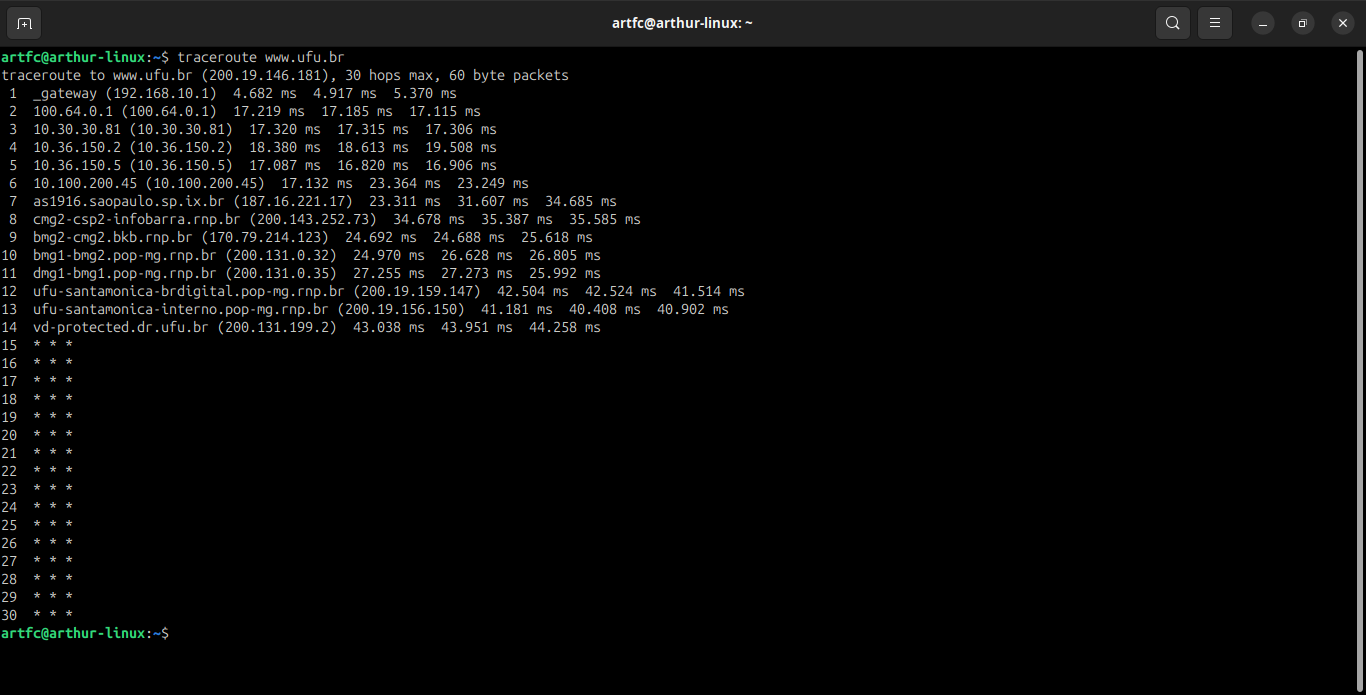
\includegraphics[width=\textwidth, keepaspectratio]{tracerouteufu.png}
				\caption{Resultado traceroute para www.ufu.br feito em CASA (Iraí de Minas)}
				\label{fig:tracerouteUFU}
			\end{figure}

			\begin{figure}[H]
				\centering
				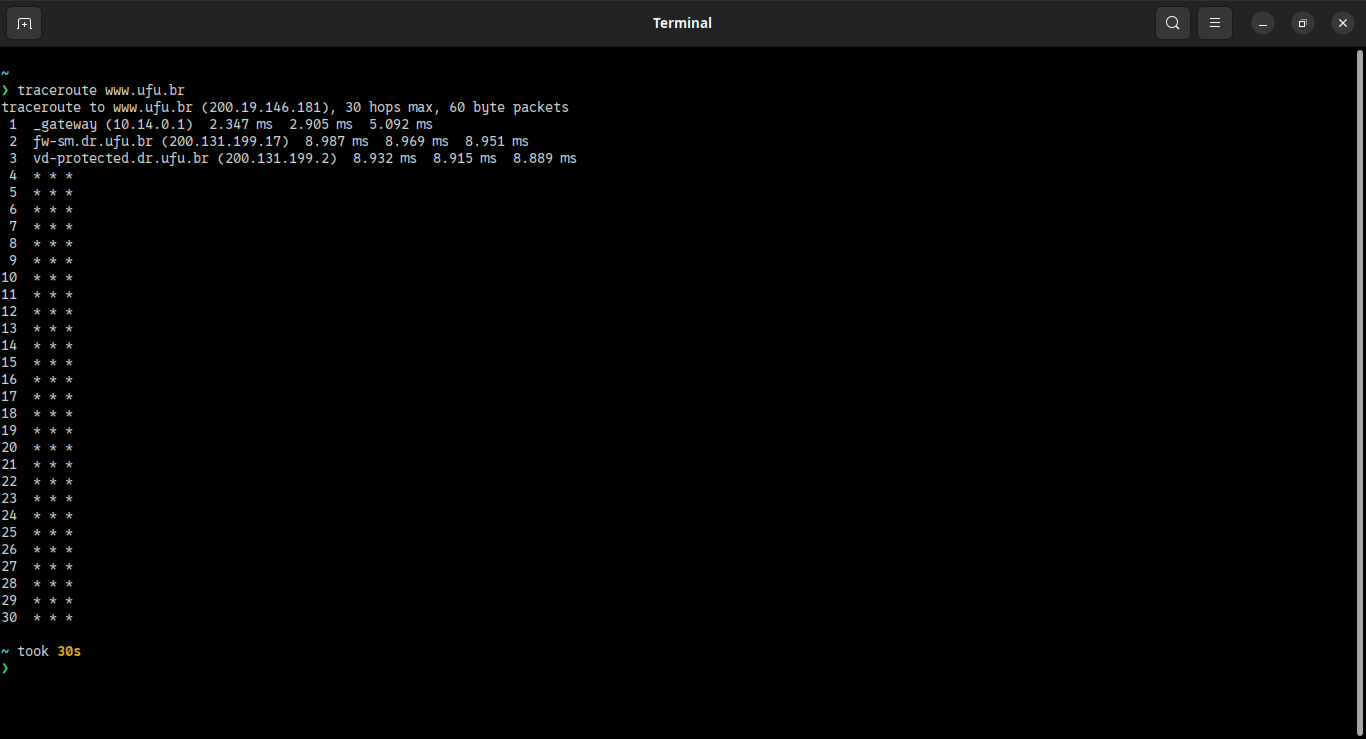
\includegraphics[width=\textwidth, keepaspectratio]{tracerouteufuufu.png}
				\caption{Resultado traceroute para www.ufu.br feito na  UFU}
				\label{fig:tracerouteUFU_UFU}
			\end{figure}

			\item O seu computador e o site www.netflix.com
			
			\begin{figure}[H]
				\centering
				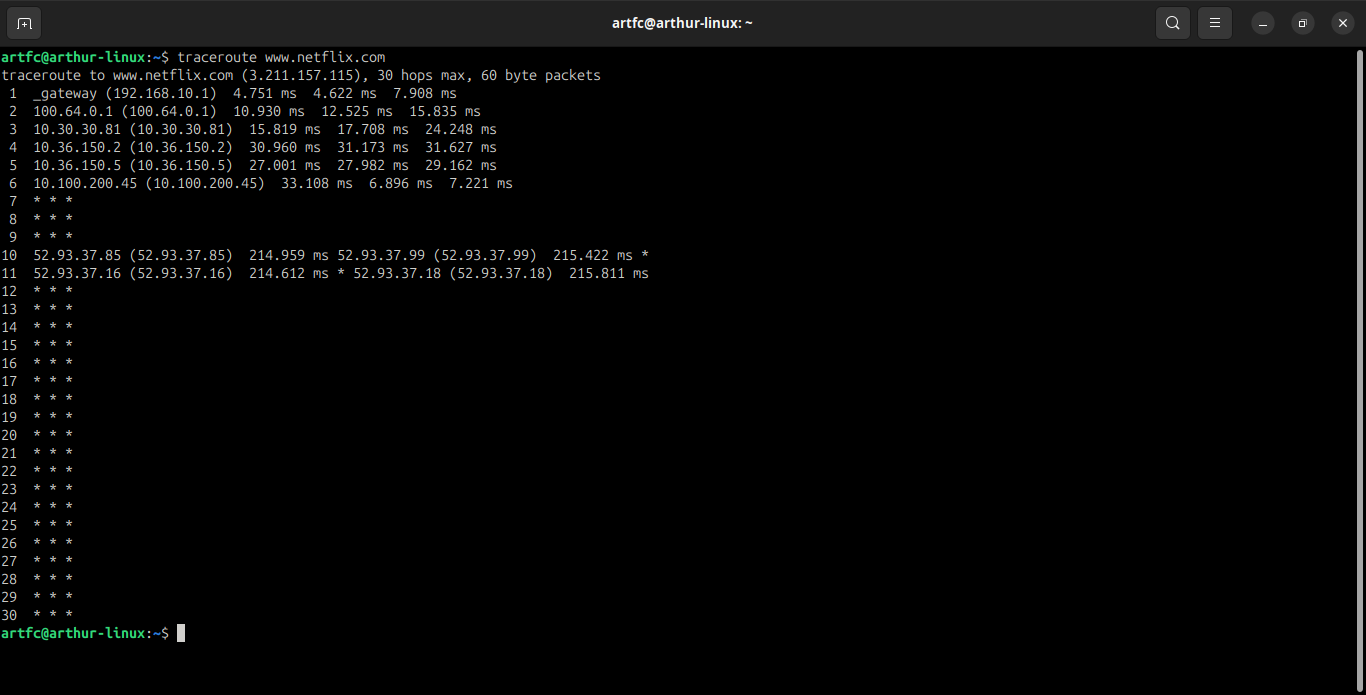
\includegraphics[width=\textwidth, keepaspectratio]{traceroutenetflix.png}
				\caption{Resultado traceroute para www.netflix.com feito em CASA (Iraí de Minas)}
				\label{fig:tracerouteNetflix}
			\end{figure}

			\begin{figure}[H]
				\centering
				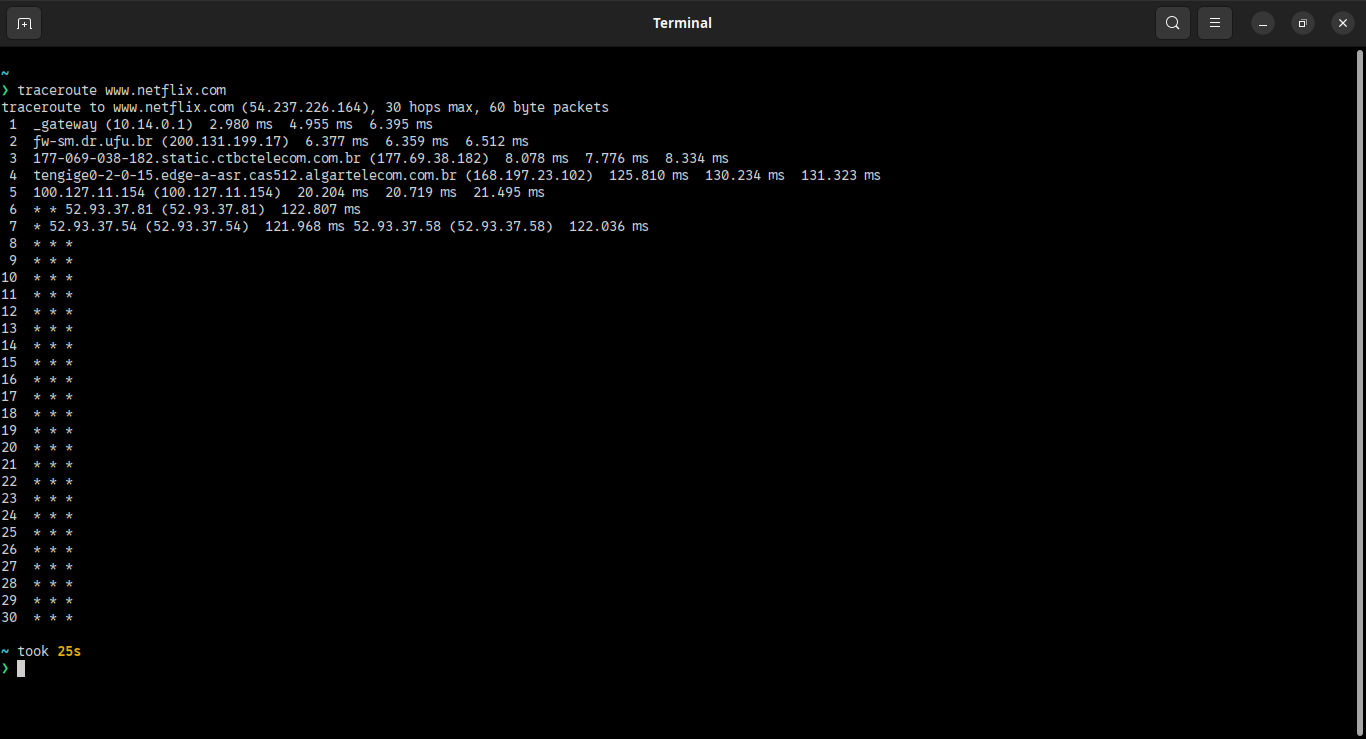
\includegraphics[width=\textwidth, keepaspectratio]{tracerouteufunetflix.png}
				\caption{Resultado traceroute para www.netflix.com feito na UFU}
				\label{fig:tracerouteNetflix_UFU}
			\end{figure}
			
			\item O seu computador e o site web.mit.edu
			
			\begin{figure}[H]
				\centering
				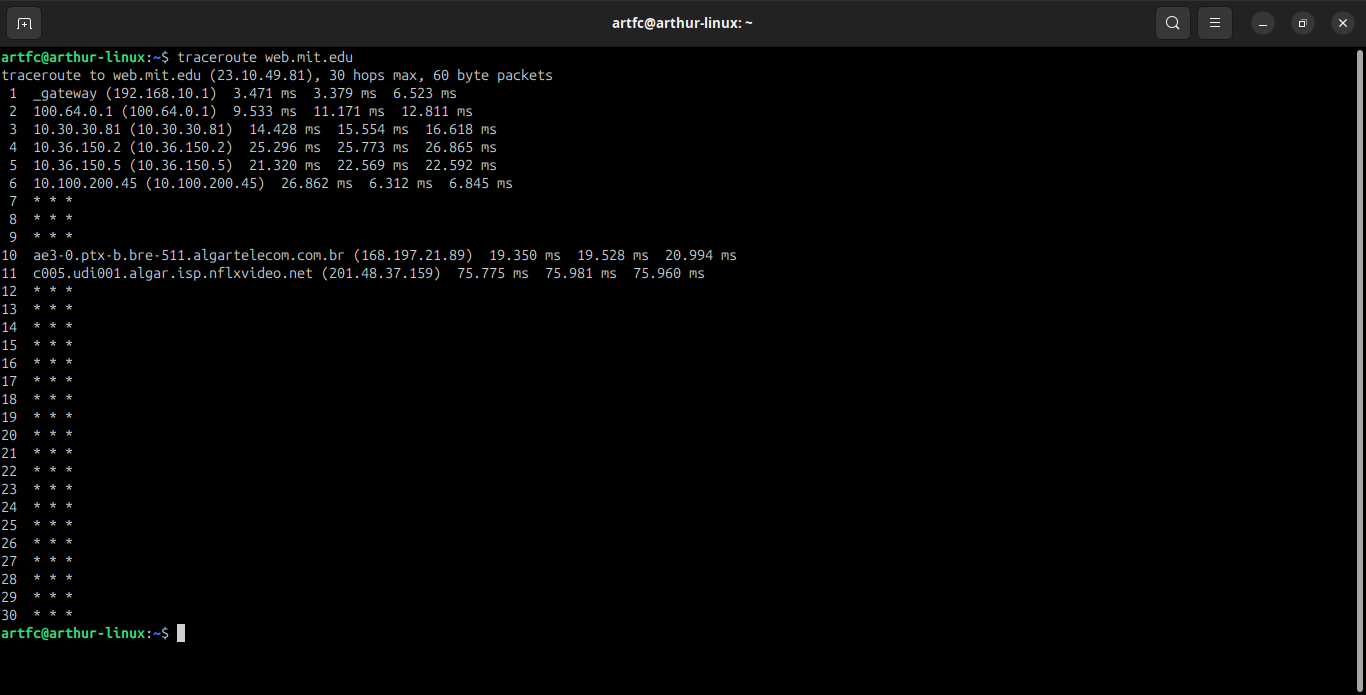
\includegraphics[width=\textwidth, keepaspectratio]{traceroutwebmit.png}
				\caption{Resultado traceroute para web.mit.edu feito em CASA (Iraí de Minas)}
				\label{fig:tracerouteWebMIT}
			\end{figure}

			\begin{figure}[H]
				\centering
				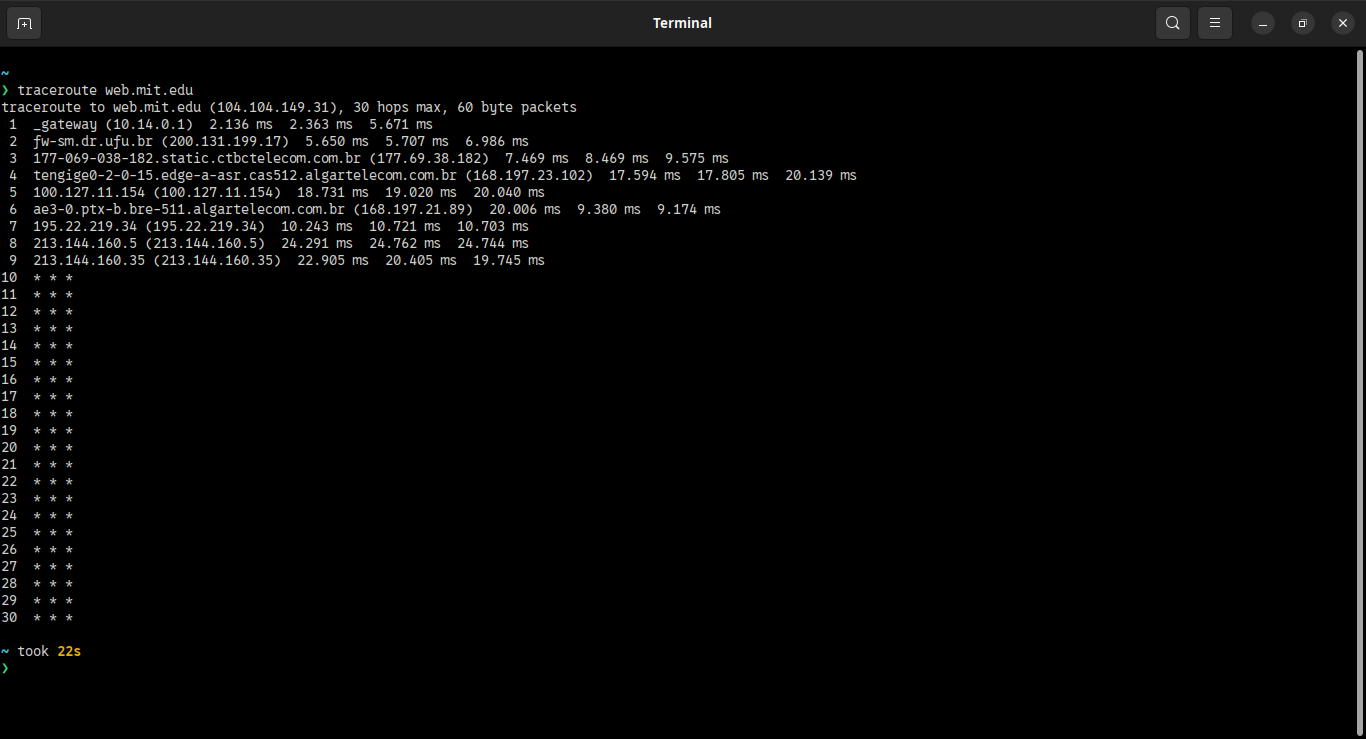
\includegraphics[width=\textwidth, keepaspectratio]{tracerouteufuwebmit.png}
				\caption{Resultado traceroute para web.mit.edu feito na UFU}
				\label{fig:tracerouteWebMIT_UFU}
			\end{figure}
			
			\item O seu computador e o site english.gov.cn
			
			\begin{figure}[H]
				\centering
				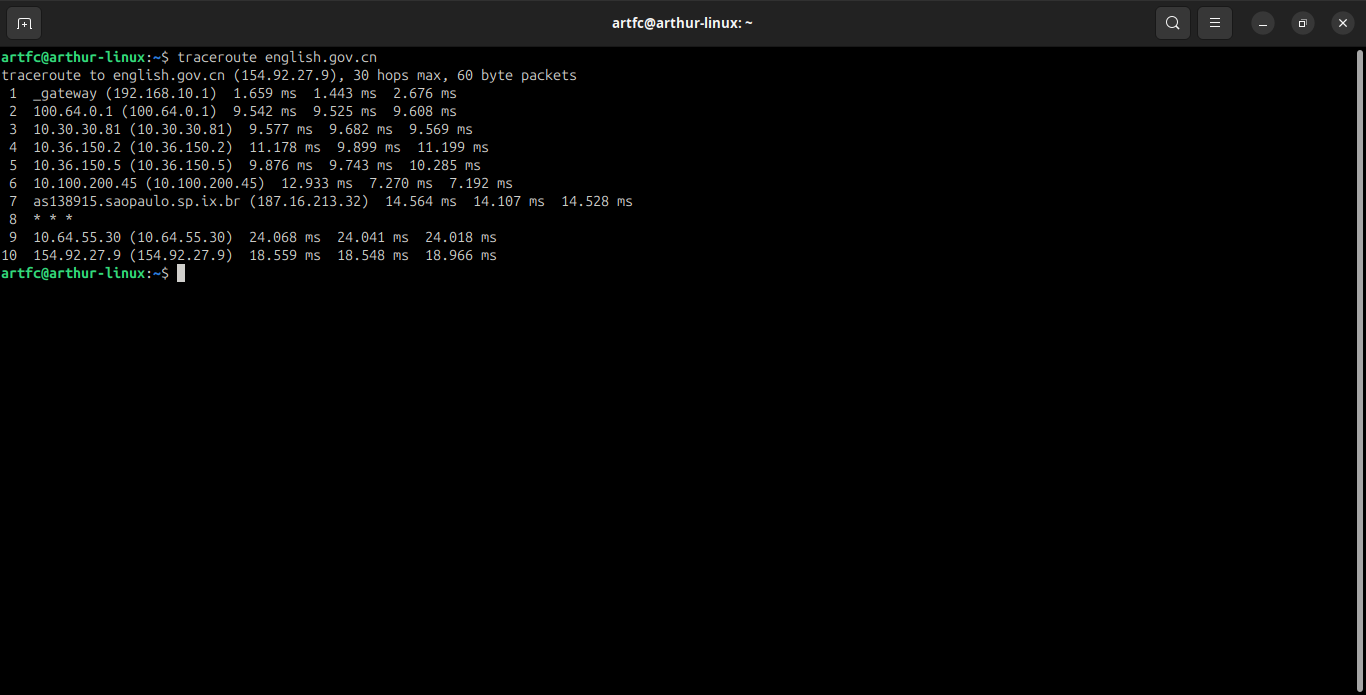
\includegraphics[width=\textwidth, keepaspectratio]{tracerouteenglish.png}
				\caption{Resultado traceroute para english.gov.cn feito em CASA (Iraí de Minas)}
				\label{fig:tracerouteEnglish}
			\end{figure}

			\begin{figure}[H]
				\centering
				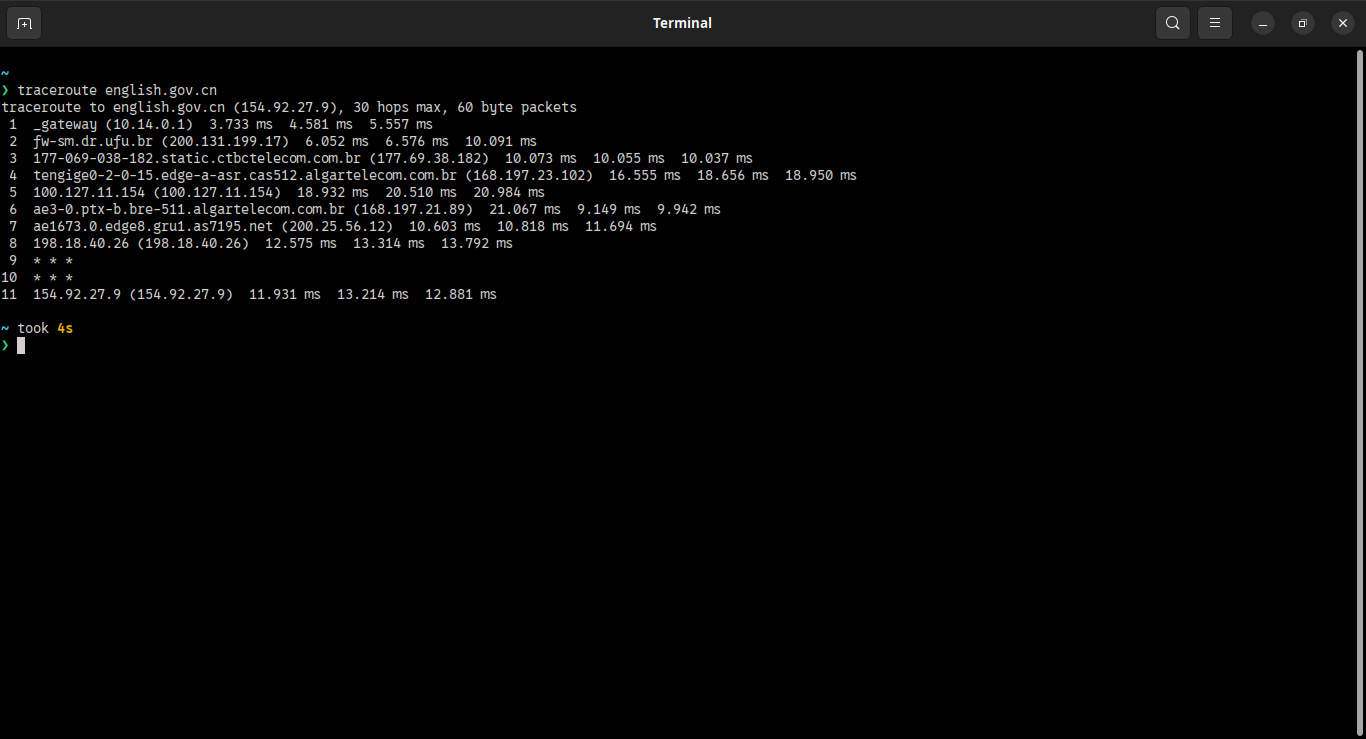
\includegraphics[width=\textwidth, keepaspectratio]{tracerouteufuenglish.png}
				\caption{Resultado traceroute para english.gov.cn feito na UFU}
				\label{fig:tracerouteEnglish_UFU}
			\end{figure}

		\end{enumerate}
		
		\item Resposta da quarta questão:

Analisando as figuras 1, 2, 3 e 4 e comparando com os meus resultados (UFU e casa) é possível notar a diferença nas saídas do comando, onde provavelmente nas figuras 1,2, 3 e 4 foram feitos em um computador com Windows, enquanto eu fiz no Linux. Além disso, praticamente em todos os casos o tempo foi menor nos meus resultados e também teve menos saltos para outros roteadores. Mesmo o meu resultado aparentando ter sido mais rápido, o meu também teve mais * que significa que o roteador alcançado foi configurado para diminuir a prioridade ou rejeitar automaticamente os pacotes ICMP (fonte do fortinet.).		

		\newpage
		\item Resposta da sexta questão:
		\begin{enumerate}[label=(\alph*)]
		\item Em ambos os casos os testes feitos na UFU foram mais rápidos, até mesmo o número de saltos foi menor para a UFU.
	
		\item Sim, o número de roteadores pode ser devido a distância em que o pacote deve percorrer até chegar ao destino, já o atraso pode ser devido a qualidade da conexão, a quantidade de pacotes que estão sendo enviados e a quantidade de pacotes que estão sendo enviados ao mesmo tempo.
		\end{enumerate}
	\end{enumerate}

\end{document}